\documentclass[11pt,a4paper]{article}
\usepackage{amsmath}
\usepackage{amsfonts}
\usepackage{amssymb}
\usepackage{graphicx}
\graphicspath{{Graphics/}} %Setting the graphicspath
\usepackage[utf8]{inputenc}
\usepackage[english]{babel}
\usepackage{lmodern}



\author{Sebastian Knigge}
\begin{document}

\section{Discussed models}

This section will introduce the reader into the two Topic modeling approaches which will be compared in this Thesis. The aim of both procedures is to assign one or more topics to different documents. Even if the vocabulary and the notation are similar for both approaches, the notation should be resumed at the beginning of the description of the respective model. The basic structural notation of the data consists of the following variables.

A collection of documents is called corpus $D=(\textbf{w}_1,\dots , \textbf{w}_M)$. It consists out of M documents $\textbf{w}=(w_1,\dots, w_N)$ which are itself separated in words $w_i$. These words are vectors of length $V$. $V$ refers to the length of a vocabulary which holds all the words occurring in the corpus. The vector for a specific word $w_i$ contains all 0 except for index $j\in\{1,...,V\}$ which represents this very one word in the vocabulary.

This notation may indeed be extended through the addition of indices for documents, but this is not done here or in the standard literature on topic models due to its unnecessary complexity.

\subsection{LDA model}
Latent Dirichlet Allocation is a Bayesian approach. The idea is based on the representation of exchangeable random variables (acc. to de Finetti) as mixture of distributions. Given that documents $\textbf{w}$ and words $w_i$ in each document - both considered as random variables in this setting - are exchangeable in such a way, a mixed model such as the LDA model are appropriate.\footnote{Cf. \cite{Blei2003}}

Let $z_j$ be the topics with $j\in\{1,\dots,k\}$. In the LDA setting we assume for e every topic $z_j$ there is a term distribution

$$\beta_j \sim Dir(\delta)$$

We further assume each document w has a distribution of topics.

$$\theta \sim Dir(\alpha)$$

Then each word $w_i$ of $\textbf{w}$ is generated by the following process:

\begin{enumerate}
	\item Choose $z_i \sim Mult(\theta)$
	
	\item Choose $w_i \sim Mult(\beta_i)$ This distribution will be referred to as $p(w_i|z_i,\beta)$
\end{enumerate}
You can summarize this setup in a plate diagram as figure \ref{PlateDiagram}.\footnote{This notation coincides with the notation of \cite{Hornik2011}}


\begin{figure}[h]
	\label{PlateDiagram}
	\centering
	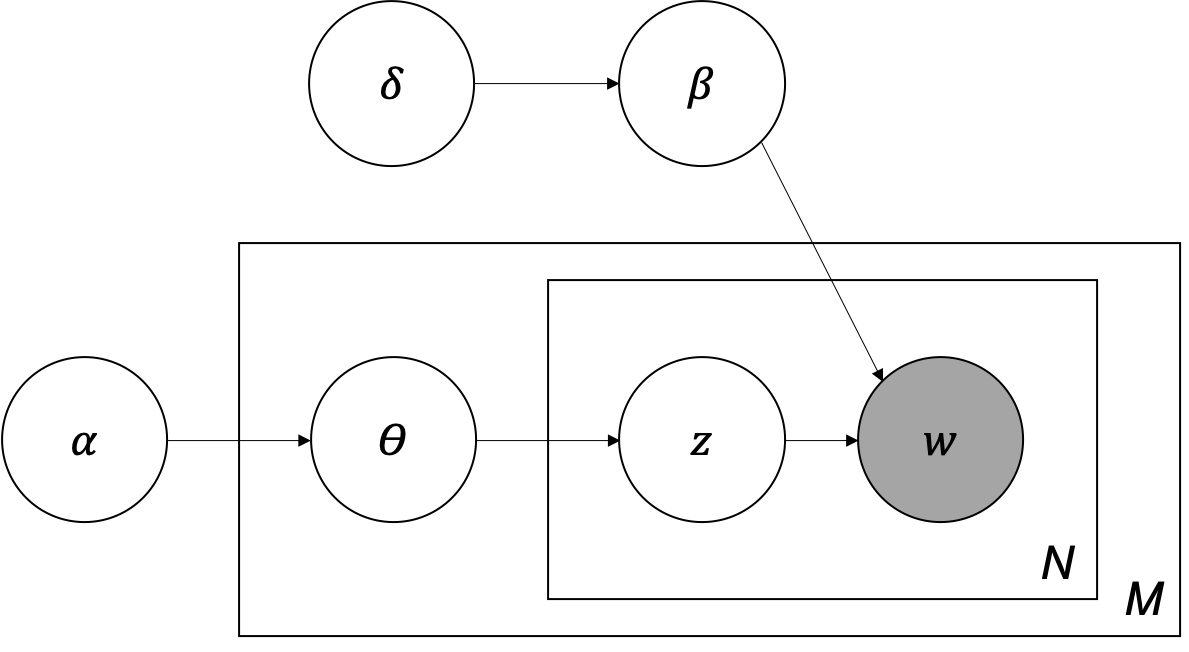
\includegraphics[width=0.5\textwidth]{LDA_Plate_Diagram.png}
	\caption{The well-established plate diagram for the standard LDA model extended by the parameter $\delta$. The slightly bigger box represents the generative model of the corporis $M$ documents. The smaller plate represents the iterative generation process of the $N$ words of each document with the aid of the topics. See also "smoothed LDA model" in \cite{Blei2003}  for comparisons.}
\end{figure}

The task now is to calculate the posterior distribution, which consists of the joint distribution in the numerator and the marginal distribution in the denominator.

\begin{align}\label{posterior}
	p(\theta,\textbf{z}|\textbf{w},\alpha,\beta)= \frac{p(\theta,\textbf{z},\textbf{w}|\alpha,\beta)}
	{p(\textbf{w}|\alpha, \beta)}
\end{align}

The joint distribution numerator can be derived straight forward.

\begin{align}\label{joint}
	p(\theta,\textbf{z},\textbf{w}|\alpha,\beta)=p(\theta|\alpha)\prod_{i=1}^{N}p(w_i|z_i,\beta)\ p(z_i|\theta)
\end{align}

One can obtain the marginal distribution of a document w, by integrating out the parameter $\theta$ and summing over the topics $z_j$. Nevertheless, this distribution is intractable.
\begin{align}\label{marginal}
p(\textbf{w}|\alpha, \beta)=\int p(\theta|\alpha) \left( \prod_{i=1}^{N} \sum_{z_i}p(z_i|\theta)p(w_n|z_i,\beta) \right) d\theta
\end{align}



	
  \bibliographystyle{apalike}
  \bibliography{MagLibrary}

	
	
\end{document}